%% LyX 2.0.5.1 created this file.  For more info, see http://www.lyx.org/.
%% Do not edit unless you really know what you are doing.
\documentclass[usenatbib]{article}
\usepackage[latin9]{inputenc}
\usepackage[a4paper]{geometry}
\geometry{verbose}
\usepackage{color}
\usepackage{graphicx}

\makeatletter

%%%%%%%%%%%%%%%%%%%%%%%%%%%%%% LyX specific LaTeX commands.
%% Because html converters don't know tabularnewline
\providecommand{\tabularnewline}{\\}
%% A simple dot to overcome graphicx limitations
\newcommand{\lyxdot}{.}


%%%%%%%%%%%%%%%%%%%%%%%%%%%%%% Textclass specific LaTeX commands.
\usepackage{jcappub}

%%%%%%%%%%%%%%%%%%%%%%%%%%%%%% User specified LaTeX commands.






%%%%%%%%%%%%%%%%%%%%%%%%%%%%%% LyX specific LaTeX commands.
%% A simple dot to overcome graphicx limitations
%Make my life significantly easier
\usepackage{lineno}
\global\long\def\bd{{\bm{\delta}}}
 \linenumbers

\makeatother

\begin{document}

\title{Generating Mock Catalogs for the Baryon Oscillation Spectroscopic
Survey: An Approximate N-Body approach}


\author{Aaronson Aardvark...e.t.c.}


\abstract{We introduce and test an approximate scheme for generating mock catalogs
for large-scale structure measurements in galaxy surveys, specializing
in this work to the Baryon Oscillation Spectroscopic Survey. things
to add later...A brief description of the approximation scheme, tests
and the accuracy we reach, and some comments about the timings of
the tests and the BOSS samples.}

\maketitle

\section{Introduction}

Recently, the necessity and the demand for the large number of large
N-body simulations have been increased in astronomy due to the precision
required for measurements to understand cosmic acceleration, like
the Baryon Oscillation Spectroscopic Survey (BOSS) and the proposed
Mid Scale-Dark Energy Spectroscopic Instrument (MS-DESI). As the area
covered by those current and future spectroscopic galaxy surveys get
larger, galaxy mocks necessary to the cosmological analysis also have
to be generated from N-body simulations with the corresponding large
volume, which is computationally expensive. Besides the large volume
required for the N-body simulations, we need many realizations to
achieve the precision required for those measurements.

There are several reasons for why we need large number of N-body simulations.
One is to understand and to calibrate systematics caused by non-linear
gravitational evolution and galaxy formation. Since those systematics
are cosmology dependent, ideally we want to generate galaxy mocks
from N-body simulations with various cosmologies. Another reason is
to reduce noise for a covariance matrix estimation. Even when 50 realizations
are used, the directly estimated covariance matrix is still noisy.
Since it is unrealistic to run N-body simulations enough number of
times to obtain a smooth directly estimated covariance matrix, there
have been several efforts to obtain a smooth covariance matrix mainly
in two directions. One approach is to estimate a covariance matrix
from theory or by fitting to a modified form of the Gaussian covariance
matrix (\textcolor{red}{citations...}). There are many different methods
to estimate, but a peculiarity common to all the methods included
in this approach requires some assumptions to compute the covariance
matrix. Those assumptions often prevent those covariance matrices
from properly accounting the effects due to non-linear gravitational
evolution such as non-gaussianities and non-localities.

Other approach is generating enough number of galaxy mocks by using
2nd Order Perturbation Theory (2LPT) and computing a covariance matrix
estimation directly (\textcolor{red}{Scoccimarro and Sheth 2002, Manera
et al. 2012, Pinocchio?}). Using 2LPT makes generation of galaxy mocks
significantly faster than the full N-body simulations, because 2LPT
allows us to compute final positions of particles only with their
initial positions without any steps in-between. The aim of our method
is the same as this approach in the sense that we want to shorten
computational time to generate those mocks. The problem of using 2LPT
is that those simulations cannot capture non-linear gravitational
evolution and therefore this approach requires to tune halo definitions
(i.e., the linking length for the Friends-of-Friends (FOF) algorithm)
and halo masses. Also, it is hard to resolve small halos in this approach,
and therefore galaxies which reside in those small halos are placed
on randomly selected dark matter particles in the mocks. It is, however,
important to keep relatively high mass resolution to understand the
systematics caused by non-linear gravitational evolution.

Our N-body simulations are consist of two components: a long time
step for solving the PM force and a set of short range sub-cycle steps
for a direct particle-particle interaction. The idea behind is reducing
the number of both time steps as much as we can preserve enough mass
resolution to correctly describe the large scale distribution of galaxies. 

In the following, we first briefly describe the mechanism of our approximated
N-body simulations. In Section 3, we test and compare our method to
the full N-body simulation and explain how we calibrate our samples.
In Section 4, we populate halos in our samples with galaxies and compute
correlation functions based on BOSS Data Release 9/11(?) geometry,
and compare it with the observed correlation function. 


\section{HACC}


\section{Convergence Test: Selection of the minimal time steps}

In this section, we examine how reducing the number of time steps
affects on halo properties (i.e., halo mass, position, and velocity)
as well as observables such as halo mass functions and halo bias.\textcolor{black}{{}
In order to quantitatively evaluate different time-stepping schemes,
we run a set of convergence tests using smaller simulation boxes.
We scale down these volumes to $(256h^{-1}{\rm Mpc})^{3}$ with $256^{3}$
particles with the same particle mass as the simulations with $(4000h^{-1}{\rm Mpc})^{3}$
. The number of time steps were chosen as 450/5, 300/3, 300/2, 150/3,
150/2, where the first number indicates the number of long time steps
and the second number the number of short time steps for each long
time step (}\textcolor{red}{Can I consider the simulations with 450/5
as the full N-body simulations or not? Also, can/should we compare
our results with the full N-body simulations?}\textcolor{black}{).
To evaluate different time-stepping schemes, we first compare the
properties (masses, positions, and velocities) of the individual halos
themselves by matching halos in one sample to halos in another. Following
to that, we compare statistical descriptions provided by the mass
functions and power spectra. We found that differences on halo properties
do not significantly affect on those statistical observables.}


\subsection{Matching }

Here, we compare halo properties by matching halos in different samples
one by one. We first show our algorithm for identifying the corresponding
halos in two different samples and then compare halo mass, position,
and velocity for those matched halos. From the quantitative comparison,
we find that the samples generated from the simulations with 300 global
steps have much less scatter for the baseline of the sample of the
450/5 simulation than the samples with 150 global steps. In addition
to that, we see that the differences between sub-cycles are almost
negligible.


\subsubsection{Algorithm}

Since our simulations all start with the same initial conditions,
we match halos in different simulations by matching their particle
content. Given a halo in simulation A, we consider the halos in simulation
B with the corresponding particles. Given this list of possible matches,
we match to the halo with the largest number of common particles.
To avoid spurious matches, we also require that the fraction of common
particles (relative to simulation A) exceeds a threshold. As an example
to illustrate how this matching algorithm works, we use the samples
from the 300/2 simulation and the 450/5 simulation. Figure \ref{fig:fraction1}
shows the cumulative fraction of unmatched halos matching the 450/5
simulation to the 300/2 simulation at $z=0.15$ with various thresholds.
As expected, the unmatched fraction increases with increasing threshold
and decreasing halo mass. We adopt a threshold of 50\% as our default
choice.

Since the above matching algorithm is unidirectional, multiple halos
in the sample A might be matched to a single halo in the sample B;
this happens 1 to 2\% of the time with a matching threshold of 50\%.
We refer to these as multiply-booked halos in what follows. Figure
\ref{fig:mass-scatter1} compares halo masses matching the 450/5 simulation
to the 300/2 simulation for the case of multiply-booked halos and
the rest. The top left panel shows a mass scatter for all the matched
halos between those two simulations, while the top right panel shows
a mass scatter onl\textcolor{black}{y for the non multiply-booked
halos}. The bottom panels show a mass scatter for the case of multiply-booked
halos. The bottom left panel shows a mass scatter for individual multiply-booked
halos, while we plots a summed halo mass for those corresponding halos
in the bottom right panel. As shown in the top left panel, there are
low-mass halos in the 450/5 simulation corresponding to high-mass
halos in the 300/2 simulation. The same trend is observed for the
case of multiply-booked halos, but not for the non multiply-booked
halos. Furthermore, those disagreement for halo masses between the
two simulations are resolved by adding the corresponding halo masses.
This implies that there are multiple halos in the 450/5 simulation
which are merged into one halo in the 300/2 simulation.

Figure \ref{fig:mass-content} shows the number densities of the unmatched
halos in the 450/5 simulation matching to the 300/2 simulation at
$z=0.15$. There are three reasons that halos are considered as unmatched.
First, if particles forming a halo in the sample A do not form a halo
in the sample B (i.e., halos in the samples do not share common particles),
we consider them as unmatched. Second, if the fraction of common particles
over the total number of particles in each halo is less than 50\%,
we eliminate halos for the case of spurious matching. At last for
the case of multiply-booked halos, we remove all but the one with
the largest number of common particles. We showed each unmatched number
density as a function of halo mass. We only find unmatched halos on
low-mass regions for the reason that the halos do not have any common
particles. This is because there are some low-mass halos which are
identified in one sample but not in another sample due to the way
the FOF algorithm define halos. As shown, most of unmatched halos
are due to the threshold criterion. \textcolor{black}{We also checked
how the number of matched halos is changed as a function of redshift,
and we observed that redshift does not affect to the matching algorithm.}

\begin{figure}
\includegraphics[width=0.5\columnwidth]{/Users/old_ts485/Dropbox/big-sims/Plots/unmatchedHalo_frac_450_300_2_z0\lyxdot 15}

\caption{\label{fig:fraction1}The cumulative fraction of unmatched halos matching
the 450/5 simulation to the 300/2 simulation at z=0.15 as a function
of halo mass. The solid lines, from top to bottom, correspond to matching
thresholds of 75\%, 50\%, and 25\% for the unmatched halos in the
450/5 sample. The dashed line shows the same quantity for the 300/2
sample for a threshold of 50\%. As expected, the unmatched fraction
increases with decreasing halo mass and increasing threshold. We adopt
a threshold of 50\% as our default choice. \textcolor{red}{Do we really
need the result for the 300/2 simulation?}}
\end{figure}


\begin{figure*}
\includegraphics[width=0.5\columnwidth]{/Users/old_ts485/Dropbox/big-sims/Plots/scatterMass_256_300_2_z0\lyxdot 15}
\includegraphics[width=0.5\columnwidth]{/Users/old_ts485/Dropbox/big-sims/Plots/testDB_nonDB_300_2_z0\lyxdot 15}

\includegraphics[width=0.5\columnwidth]{/Users/old_ts485/Dropbox/big-sims/Plots/testDB_DB_numPartCut_300_2_z0\lyxdot 15}
\includegraphics[width=0.5\columnwidth]{/Users/old_ts485/Dropbox/big-sims/Plots/testDB_sum_mass_f0\lyxdot 5_300_2_z0\lyxdot 15}

\caption{\label{fig:mass-scatter1}Comparison of halo masses matching the 450/5
simulation (x-axis) to the 300/2 simulation (y-axis) at $z=0.15$.
Panels correspond to halos with different matching criteria: all the
matched halos (top left), matched halos having one-to-one correspondence
(top right), matched halos not having one-to-one correspondence called
``multiply-booked'' halos (bottom left), and the ``multiply-booked''
halos whose corresponding halo masses are added (bottom right). Those
panels imply that large mass difference between the 450/5 simulation
and the 300/2 simulation shown in the top left panel is mainly because
those ``multiply-booked'' halos in the 450/5 simulation are merged
into one halo in the 300/2 simulation due to larger time steps.}
\end{figure*}


\begin{figure}
\includegraphics[width=0.5\columnwidth]{/Users/old_ts485/Dropbox/big-sims/Plots/unmatchHalo2_content_300_2_z0\lyxdot 15}

\caption{\label{fig:mass-content} Itemization of unmatched halos shown as
cumulative number densities of the unmatched halos from each procedure
in the matching algorithm. The solid line is the total and the dashed
lines correspond to matching based on particle content (green), elimination
due to the matching threshold (red), and elimination of ``multiply-booked''
halos (cyan). Most large halos being unmatched is due to the threshold. }
\end{figure}



\subsubsection{Halo Properties}

Here, we compare halo properties (i.e., halo mass, position, and velocity)
for halos matched to those in the 450/5 simulation. Since we are interested
in correctly describing the large-scale distribution of galaxies and
it requires to correctly locate dark matter halos in the simulation
with correct estimation of halo masses, it is crucial to know how
reducing the number of time steps affects on halo properties systematically.
The comparison of halo mass for different time-stepping schemes to
the 450/5 simulation at $z=0.15$ is shown in Figure \ref{fig:HaloProperty_mass}.
We take all the matched halos whose masses are between $10^{12.5}{\rm M_{\odot}}$
to $10^{13.0}{\rm M_{\odot}}$, $10^{13.0}{\rm M_{\odot}}$ to $10^{13.5}{\rm M_{\odot}}$,
and $10^{13.5}{\rm M_{\odot}}$ to $10^{14.0}{\rm M_{\odot}}$, and
compute their means and the standard deviations for ${\rm log_{10}(M/M_{450/5})}$,
where $M_{450/5}$ is a halo mass for the 450/5 simulation and $M$
corresponds to a halo in the samples generated with different time-stepping
schemes. Figure \ref{fig:HaloProperty_mass} shows that halos generated
from the simulations with small number of time steps have systematically
lower masses than those in the 450/5 simulation. This is partly because
we use the same linking length for the FOF algorithm to define halos
for all the simulations. Since reducing the number of time steps results
in an approximation to the true dynamics of dark matter fields, halos
in the 450/5 simulation tend to have tighter and denser structure
(\textcolor{red}{show the snapshot?}). So, using the same linking
length will miss connecting some particles in the simulations with
small number of time steps and will result in smaller halos than the
corresponding halo in the 450/5 simulation. The panels in Figure \ref{fig:HaloProperty_step},
from left to right, show the comparison of halo position and velocity
for the matched halos at $z=0.15$. As shown, the 150 global steps
have more scatter in the halo positions and the means d\textcolor{black}{iffer
for} the velocity difference. For the 300 global steps, the results
are significantly improved and the center position is matched in these
cases to better than 200 kpc. As is clear from Figure \ref{fig:HaloProperty_step},
the difference between 3 and 2 sub-cycles is negligible on halo properties.
Note that we observe the same trend in halo properties discussed here
at different redshifts.

\begin{figure}[t]
\includegraphics[width=0.5\columnwidth]{/Users/old_ts485/Dropbox/Tomomi/HACC/Conv/Test_correction/massSlice_z0\lyxdot 15}

\caption{\label{fig:HaloProperty_mass}Comparison of halo mass for matched
halos between the 450/5 simulation and other time-stepping schemes
at $z=0.15$. We take all the matched halos whose masses are between
$10^{12.5}{\rm M_{\odot}}$ to $10^{13.0}{\rm M_{\odot}}$, $10^{13.0}{\rm M_{\odot}}$
to $10^{13.5}{\rm M_{\odot}}$, and $10^{13.5}{\rm M_{\odot}}$ to
$10^{14.0}{\rm M_{\odot}}$, and compute the mean and the standard
deviation for ${\rm log_{10}(M/M_{450/5})}$ where $M_{450/5}$ is
a halo mass for the 450/5 simulation and $M$ is for the simulations
with different number of time steps corresponding to different colors
in the plot. This plot shows that halo masses become systematically
smaller for the case of small number of time steps than those in the
450/5 simulation.}
\end{figure}


\begin{figure*}[t]
\includegraphics[width=0.5\columnwidth]{/Users/old_ts485/Dropbox/big-sims/Plots/histogram_distance_z0\lyxdot 15}\includegraphics[width=0.5\columnwidth]{/Users/old_ts485/Dropbox/big-sims/Plots/histogram_velocity_z0\lyxdot 15}

\caption{\label{fig:HaloProperty_step}Comparison of matched halos in the different
simulations corresponding to the time steps of 300/3 (blue), 300/2
(green), 150/3 (red), and 150/2 (cyan) with respect to the 450/5 simulation.
From left to right, we compared halo position and velocity respectively.\textcolor{blue}{{}
}\textcolor{black}{The agreement between 300 global steps and the
450/5 simulation is considerably good, with little difference from
the number of sub-cycles.}}
\end{figure*}



\subsection{Mass Adjustment}

In the previous subsection, Figure \ref{fig:HaloProperty_mass} shows
that halos generated by the de-tuned simulations have systematically
lower masses than the halos in the 450/5 simulation. This suggests
the necessity of adjusting halo masses for those cases to the halo
masses in the 450/5 simulation. In the following, we describe how
we do a mass adjustment and show the resulted observables including
mass functions and power spectra.


\subsubsection{Method}

To calibrate halo masses for the simulations with the reduced number
of time steps, we first take all the matched halos between the 450/5
simulation and the de-tuned simulations and compute means for each
mass bin. The reason we only take the matched halos is because our
purpose of mass adjustment here is to correct systematic mass differences
for the halos which are theoretically identical in different samples.
After computing the means for each mass bin, we fit those means to
a functional shown below so that $M_{re}$ becomes close to the average
halo masses for the 450/5 simulation:

\begin{equation}
M_{re}=M(1.0+\alpha(M/10^{12.0}[{\rm M_{\odot}])^{\beta},}\label{eq:mass_adjust}
\end{equation}
where $M_{re}$ is a reassigned halo mass, $M$ is an original halo
mass, $\alpha$ and $\beta$ are free parameters. Corresponding $\alpha$
and $\beta$ for the simulations with different number of time steps
at $z=0.15$ are listed on Table \ref{tab:free_param1}.

\begin{table}
\begin{tabular}{|c|c|c|}
\hline 
 & $\alpha$ & $\beta$\tabularnewline
\hline 
\hline 
300/3 & 0.005 & 0.175\tabularnewline
\hline 
300/2 & 0.07 & -0.47\tabularnewline
\hline 
150/3 & 0.101 & -0.162\tabularnewline
\hline 
150/2 & 0.315 & -0.411\tabularnewline
\hline 
\end{tabular}

\caption{\label{tab:free_param1}Corresponding $\alpha$ and $\beta$ in Eq.
\ref{eq:mass_adjust} for the samples with different number of time
steps at $z=0.15$.}


\end{table}


Those free parameters $\alpha$ and $\beta$ can be described as a
function of redshift. For the case of the 300/2 simulation as an example,
we find best fit parameters shown below (\textcolor{red}{any examples
or plots for here? How can I tell the readers that this mass adjustment
is successful more quantitatively?}):

\begin{equation}
\alpha(z)=0.123z+0.052,
\end{equation}
and
\begin{equation}
\beta(z)=-0.154z-0.447.
\end{equation}



\subsubsection{Observables}

Now, we show mass functions and power spectra for the different simulations
after applying the mass adjustment.

We first compute mass functions from outputs of different time-stepping
schemes, as shown in Figure \ref{fig:massFn_step}, where we compare
simulations with reduced number of time steps to the 450/5 simulation
at $z=0.15$. In Figure \ref{fig:massFn_step}, we show the ratio
$n(>M)/n_{450/5}(>M)$, where $n_{450/5}(>M)$ is a cumulative mass
function for the 450/5 simulation and $n(>M)$ is a cumulative mass
function for different time steps shown in different colors. We compare
the results before and after mass adjustment (left and right panels
respectively). While the mass functions from the 250/3 and 150/2 simulations
are suppressed more than10\% on all mass ranges before mass adjustment,
they are significantly improved after mass adjustment, especially
on halo masses greater than $10^{13.0}{\rm M_{\odot}}$. For the simulations
with the 300 global time steps, mass adjustment is especially effective
on small halo masses.

\begin{figure}
\includegraphics[width=0.5\columnwidth]{/Users/old_ts485/Dropbox/big-sims/Plots/haloRatioNum256_z0\lyxdot 15}\includegraphics[width=0.5\columnwidth]{/Users/old_ts485/Dropbox/Tomomi/HACC/Conv/Test_correction/haloRatioNum256_tweak_z0\lyxdot 15}

\caption{\label{fig:massFn_step} Comparison of cumulative mass functions in
different simulations taking the 450/5 simulation as a reference.
Lines, from top to bottom, correspond to the simulation with different
time steps, 300/3 (blue), 300/2 (green), 150/3 (red), and 150/2 (cyan)
respectively. A left panel shows the cumulative mass functions before
mass adjustment, and a right panel is after mass adjustment. Those
plots indicate that a systematic mass adjustment successfully calibrate
halo masses for the de-tuned simulations, even for the case of the
150/2 simulation, which has more than 10\% discrepancy before the
mass adjustment. }
\end{figure}


The next measure of interest is halo-matter cross power spectra between
halo and matter density fields, as shown in Figure \ref{fig:crossMater_step}.
Figure \ref{fig:crossMater_step} shows the ratio $P_{hm}/P_{hm,450/5}$
at $z=0.15$, where $P_{hm,450/5}$ is the cross power spectrum for
the 450/5 simulation and $P_{hm}$ is the cross power spectrum for
other time steps corresponding to different colors, as labeled in
Figure \ref{fig:crossMater_step}. We use the real-space halo density
field for the left panel and the redshift-space halo densities for
the right panel in Figure \ref{fig:crossMater_step}. For the dark
matter density field, we use the output of the 450/5 simulation for
all the halo samples. Note that the dark matter density fields are
in real-space for both cases. In this way, the ratio $P_{hm}/P_{hm,450/5}$
in real-space i\textcolor{black}{s equivalent to the ratio of halo
bias between the 450/5 simulation and the simulations with other time-steps.
To select halos, we apply the soft-mass cut method using the probability
given by }

\textcolor{black}{
\begin{equation}
<N_{halo}(M)>=\frac{1}{2}{\rm erfc}(\frac{{\rm log(M_{cut}/}M)}{\sqrt{2}\sigma}),
\end{equation}
where we set ${\rm M_{cut}=10^{13.0}[{\rm M_{\odot}]}}$ and $\sigma=0.5$.
This probability has a similar form to the halo occupation distribution
(hereafter, HOD) technique so that the probability gradually becomes
one as increasing halo mass. We use this method to avoid noise from
halos scattering across sharp boundaries on halo mass.}\textcolor{red}{{}
}Note that the errors calculated here are not due to sample variance,
because we generate 10 samples from one full sample by using the soft-mass
cut method. We see that, as we decrease the number of time steps,
the ratio of the cross power spectra increases, especially in redshift-space,
we observe large deviations from one on small scales for the 150/2
and 150/3 simulations. This is due to the overall smaller halo velocities
for those simulations, which is shown in Figure \ref{fig:HaloProperty_step}.
For the simulations with the 300 global time steps, overall agreements
with the 450/5 simulation are almost 1\% on any scales in both real-space
and redshift-space.

\begin{figure*}[p]
\includegraphics[width=0.5\columnwidth]{/Users/old_ts485/Dropbox/big-sims/Plots/crossMatter_tweak256_real_z0\lyxdot 15}\includegraphics[width=0.5\columnwidth]{/Users/old_ts485/Dropbox/big-sims/Plots/crossMatter_tweak256_redshift_z0\lyxdot 15}

\caption{\label{fig:crossMater_step} Ratio of halo-matter cross pow\textcolor{black}{er
spectra as a function of time steps with respect to the 450/5 simulation
at $z=0.15$. We use the real-space halo density field for the left
panel and the redshift-space halo density field for the right panel,
while the dark matter density fields used here are in real-space for
both cases. The left panel shows that agreements with the 450/5 simulation
are all within 2\%. In the right panel, the large discrepancy of the
cross power spectra for the simulations with 150 global steps on small
scales is mainly due to the systematically small velocities, as shown
in Figure \ref{fig:HaloProperty_step}. Note that the halos are selected
based on the soft mass-cut method with $M_{cut}=13.0$ and $\sigma=0.5$.}}
\end{figure*}


As a conclusion through several convergence tests shown in this section,
we find that the observables such as mass functions and power spectra
are not affected by the differences on halo properties as much as
those systematic differences (\textcolor{red}{better way to phrase?}).


\section{THE BOSS SIMULATIONS}
\begin{itemize}
\item Simulation Parameters: Nikhil
\end{itemize}
describe box size, masses, geometry etc. Show that we can fit in two
BOSS volumes per box. Also, mention that we decide to use the 300/2
simulations (as an example here).


\subsection{Building the Galaxy Catalog}

To generate galaxy mock catalogs, we need to go through the following
steps:

1) populate halos with galaxies through the HOD functional form,

2) give positions and velocities to the galaxies assuming an NFW profile
(\textcolor{red}{Navarro, Frenk \& White 1996}).

The HOD functional form gives probabilities for the number of central
and satellite galaxies based on mass of halos which host those galaxies
with five free parameters. For each halo, the number of central galaxies
is either 0 or 1 given by $N_{cen}(M)$, and the number of satellite
galaxies is given by Poisson distribution with a mean $N_{sat}(M)$:

\begin{equation}
N_{cen}(M)=\frac{1}{2}{\rm erfc}\left[\frac{{\rm ln}(M_{cut}/M)}{\sqrt{2}\sigma}\right],
\end{equation}
and
\begin{equation}
N_{sat}(M)=N_{cen}(M)\left(\frac{M-\kappa M_{cut}}{M_{1}}\right)^{\alpha},
\end{equation}
where $M_{cut}$, $M_{1}$, $\sigma$, $\kappa$, and $\alpha$ are
free parameters and $M$ is a halo mass. Note that $N_{sat}(M)$ is
zero when $M<\kappa M_{cut}$. Note that halos do not host satellite
galaxies without a central galaxy. The total number of galaxies hosted
by each halo is a sum of the number of central and satellite galaxies.
There are several different functional forms used in different papers,
but there is little difference on distribution of central and satellite
galaxies between those different functionals.

Now, we need to give positions and velocities to those populated galaxies.
For central galaxies, their positions are always at the center of
the halos and their velocities are the same as the velocities of the
halos hosting those central galaxies. For satellite galaxies, we place
them randomly assuming the NFW profile:
\begin{equation}
\rho(r)=\frac{4\rho_{s}}{\frac{r}{r_{s}}(1+\frac{r}{r_{s}})},
\end{equation}
where $r_{s}$ is the characteristic radius defined as $r_{s}=R_{vir}/c$,
where $R_{vir}$ is a virial radius for a halo and $c$ is the concentration
parameter. The distance $r$ from the center of the halo is given
by the probability based on the NFW profile. There have been several
studies how to describe the concentration parameter $c$ as a function
of halo mass and redshift (\textcolor{red}{citations}). In this paper,
we used the formula presented in \textcolor{red}{Klypin et al. 2010}:
\begin{equation}
c(M,z)=\frac{c_{0}}{1+z}(M-M_{0})^{-\beta},
\end{equation}
where$c_{0}=9.60$, $M_{0}=10^{12.}$, and $\beta=0.75$. 

We assign velocities to the satellite galaxies by using the virial
theorem. The virial theorem states that the mean kinetic energy of
the system is equivalent to half the mean potential energy, as shown
below:

\begin{equation}
<v^{2}>=\frac{GM}{R_{vir}}.\label{eq:variance}
\end{equation}
We draw a Gaussian distribution with zero mean and variance in Eq.
\ref{eq:variance} to give an internal velocity for the satellite
galaxies. Here, we assume that satellite galaxies are randomly moving
inside the host halos. So, we give the radial component of this random
motion from the Gaussian distribution and determine the direction
randomly with equal probability. Note that the total velocity of the
satellite galaxies is given as the sum of the halo velocity at the
center of the host halo and the velocity contributed as a random motion
inside the halo.

Now, we generate galaxy mocks with our samples at $z=0.55$. In Figure
\ref{fig:xis}, we compare the correlations function $\xi(s)$ with
the one in \textcolor{red}{Anderson et al. (2013)}\textcolor{black}{,
where $s$ is the redshift-space coordinate. Here, we use the following
HOD parameters:}

\textcolor{black}{$M_{cut}=12.9$, }

\textcolor{black}{$M_{1}=14.05$, }

$\alpha=0.9$,

\textcolor{black}{$\kappa=1.13$, }

\textcolor{black}{$\sigma=0.74$. }

\textcolor{red}{Note that we compute the correlation functions in
the redshift-space with periodic boundary condition (If we decide
to use the correlation function computed after cutting out and fitting
to n(z), I need to change this part). }\textcolor{black}{The correlation
function computed from our sample mocks fits to the correlation function
in Anderson et al. 2013 well on the scale between $30h^{-1}{\rm Mpc}$
and $80h^{-1}{\rm Mpc}$. Due to the large smoothing scale (i.e.,
the grid size used to compute $\xi(s)$ is about $8h^{-1}{\rm Mpc}$),
our BAO peak is more smoothed out than the one in Anderson et al.
2013.}

\begin{figure}
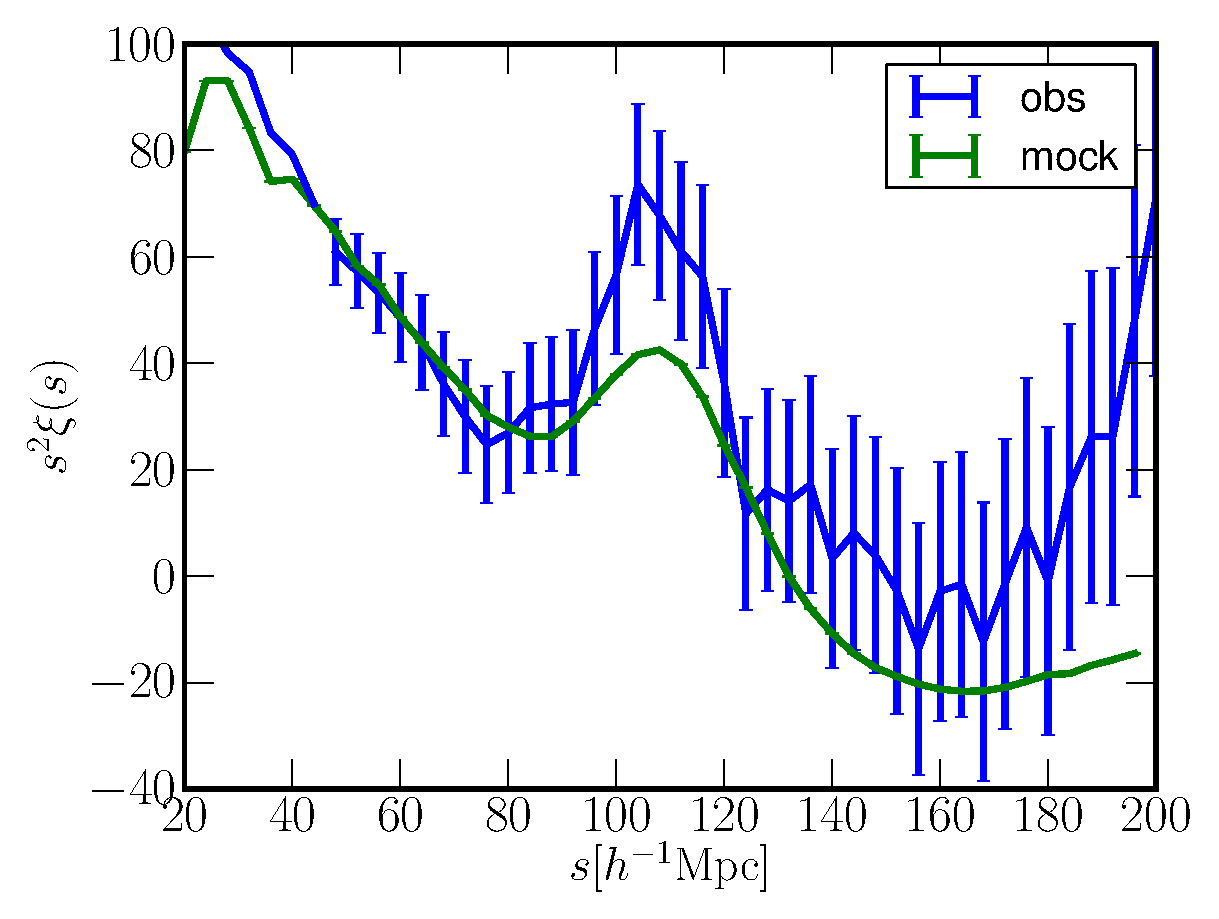
\includegraphics[width=0.5\columnwidth]{/Users/old_ts485/Dropbox/big-sims/Plots/xis_obs_wError}

\caption{\label{fig:xis}Correlation function monopoles $\xi(s)$ of the mocks
(green) and of the CMASS galaxy measured in \textcolor{red}{Anderson
et al. (2013)} (blue) at $z=0.55$. The BAO peak of the mock correlation
function is smoothed due to the wide window function.}


\end{figure}



\section{Discussion and Summary}

In this paper, we study how reducing the number of time steps in the
N-body simulations affects halo properties and statistical observables
computed from the mocks generated by those approximated N-body simulations.
Through several convergence tests described in Section 3, we find
that systematic differences on halo properties due to the approximated
gravitational dynamics give little effects on statistical observables.
Especially, the agreement between the full N-body simulation (i.e.,
the 450/5 simulation) and the approximated simulations on halo bias
is within 1\textasciitilde{}2\% after the mass adjustment. In Section
4, we generate galaxy mocks from the sample of the 300/2 simulation
at $z=0.55$ in order to compare our result with the correlation function
appeared in \textcolor{red}{Anderson et al. 2013}. The overall agreement
on the scale between $30h^{-1}{\rm Mpc}$ and $80h^{-1}{\rm Mpc}$
is well within the error in the measurement. 

From the results we show in this paper, we conclude that the approximated
N-body simulations can capture necessary physics to the current and
future galaxy spectroscopic surveys and will be effective enough to
achieve the precision required to those surveys.
\end{document}
